\documentclass[tikz,border=5mm]{standalone}
\usetikzlibrary{decorations.markings}

\begin{document}
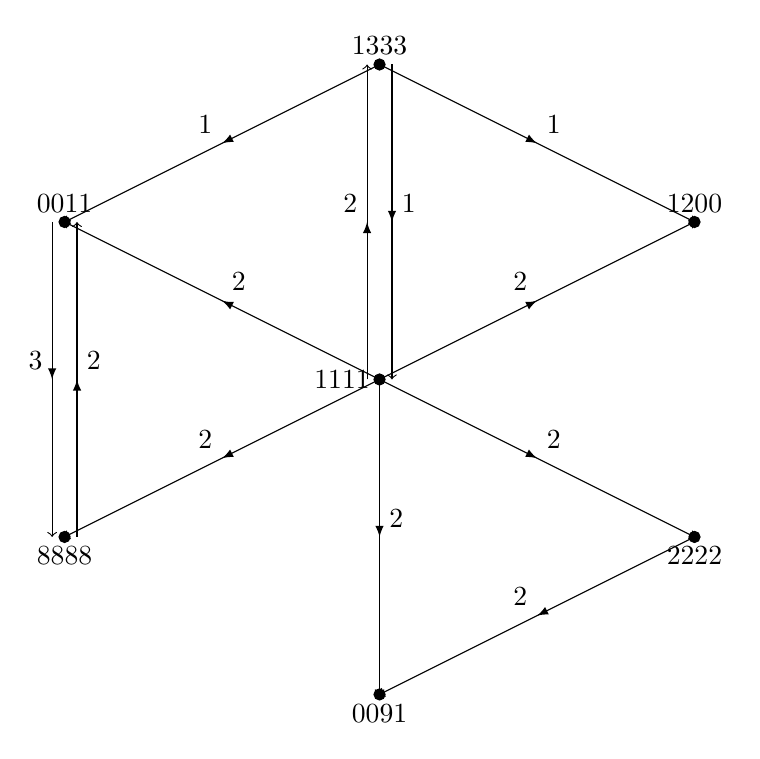
\begin{tikzpicture}
    \tikzset{
        myarrow/.style={
            postaction={
                decorate,
                decoration={
                    markings,
                    mark=at position #1 with {\arrow{latex}},
                },
            },
        },
    }

    % Vertices
    \draw[fill=black] (6,  6) circle (2pt) node[left] {$1111$};
    \draw[fill=black] (6, 10) circle (2pt) node[above] {$1333$};
    \draw[fill=black] (6,  2) circle (2pt) node[below] {$0091$};
    \draw[fill=black] (2,  8) circle (2pt) node[above] {$0011$};
    \draw[fill=black] (10, 8) circle (2pt) node[above] {$1200$};
    \draw[fill=black] (2,  4) circle (2pt) node[below] {$8888$};
    \draw[fill=black] (10, 4) circle (2pt) node[below] {$2222$};

    % Arcs
    \draw[->, myarrow=.5, transform canvas={xshift=-4.5pt}] (6,6) -- node[midway, above left] {2}  (6,10);
    \draw[->, myarrow=.5] (6,6) -- node[midway, above right] {2}  (6,2);
    \draw[->, myarrow=.5] (6,6) -- node[midway, above right] {2}  (2,8);
    \draw[->, myarrow=.5] (6,6) -- node[midway, above left] {2}  (10,8);
    \draw[->, myarrow=.5] (6,6) -- node[midway, above left] {2}  (2,4);
    \draw[->, myarrow=.5] (6,6) -- node[midway, above right] {2}  (10,4);
    \draw[->, myarrow=.5, transform canvas={xshift=-4.5pt}] (2,8) -- node[midway, above left] {3}  (2,4);
    \draw[->, myarrow=.5, transform canvas={xshift=4.5pt}] (2,4) -- node[midway, above right] {2}  (2,8);
    \draw[->, myarrow=.5] (10,4) -- node[midway, above left] {2}  (6,2);
    \draw[->, myarrow=.5] (6,10) -- node[midway, above left] {1}  (2,8);
    \draw[->, myarrow=.5, transform canvas={xshift=4.5pt}] (6,10) -- node[midway, above right] {1}  (6,6);
    \draw[->, myarrow=.5] (6,10) -- node[midway, above right] {1}  (10,8);
\end{tikzpicture}
\end{document}
